\problemname{Tivoli}

Lisa har kommit till tivolit och har bestämt vilka $N$ attraktioner hon vill åka, hon vill åka varje attraktion en gång.
För varje attraktion finns det två stycken anläggningar som är likvärdiga, det finns alltså totalt $2N$ anläggningar.
Givet positionerna för samtliga anläggninar, hjälp Lisa att planera vilka $N$ anläggningar hon ska välja och i vilken ordning för att minimera den sträcka hon måste gå för att ha åkt alla $N$ attraktioner.

Hon börjar dessutom vid entrén och ska också sluta där. Entrén är vid origo, $(0, 0)$.

\begin{figure}[h]
    \centering
    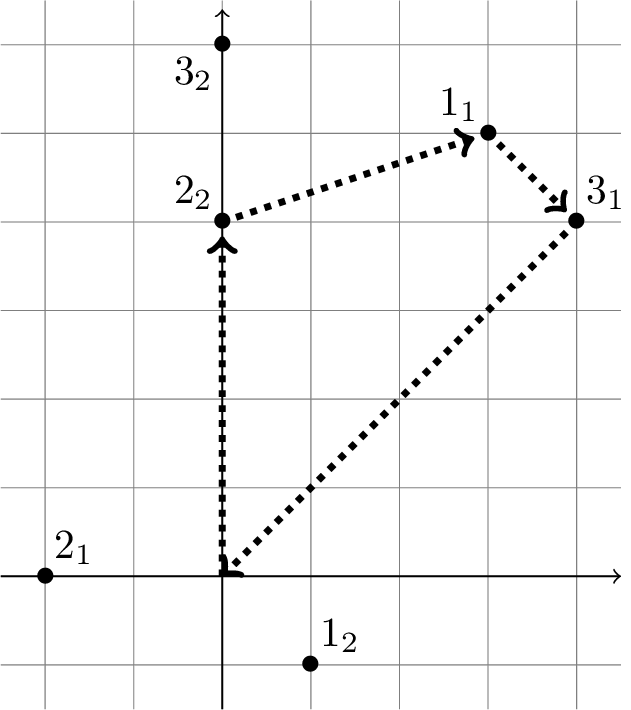
\includegraphics[width=0.2\textwidth]{tivoli}
    \caption{En illustration av det första exempelfallet och en optimala lösningen.}
\end{figure}

\section*{Indata}
Första raden består av heltalet $N$, antalet attraktioner Lisa vill åka ($1 \le N \le 15$).
Därefter följer $N$ rader, där den första raden beskriver attraktion nummer $1$, den andra raden attraktion nummer $2$ o.s.v.
Varje rad innehåller fyra heltal: x- och y-koordinat för den första anläggningen av denna attraktion, samt x- och y-koordinat för den andra anläggningen av denna attraktion.
Koordinaternas absolutbelopp understiger en miljon.

Ingen anläggning är på samma plats som en annan, eller på origo.

\section*{Utdata}
Den första raden av utdatan ska bestå av ett flyttal: hur långt Lisa måste gå.
Därefter ska $N$ rader följa med två heltal vardera, varav det första inom (mellan $1$ och $N$) säger vilken attraktion hon ska gå till, och det andra inom ($1$ eller $2$) vilken av anläggningarna.

Om det finns flera vägar som ger lika kort sträcka (det finns ju åtminstone alltid två håll att gå) kan du ange vilken som helst av dem.

Det relativa eller absoluta felet ska understiga $10^{-5}$.

\section*{Poängsättning}
Din lösning kommer att testas på en mängd testfallsgrupper.
För att få poäng för en grupp så måste du klara alla testfall i gruppen.

\noindent
\begin{tabular}{| l | l | p{12cm} |}
  \hline
  \textbf{Grupp} & \textbf{Poäng} & \textbf{Gränser} \\ \hline
  $1$    & $20$        & $N \le 1$ \\ \hline 
  $2$    & $40$        & $N \le 5$ \\ \hline
  $3$    & $40$        & Inga ytterligare begränsningar. \\ \hline 
\end{tabular}
